\documentclass[11pt,letterpaper]{article}
\usepackage[margin=1in]{geometry}
\usepackage{graphicx,amsmath,amssymb,booktabs,hyperref,tikz,pgfplots}
\usetikzlibrary{arrows.meta,positioning,fit,backgrounds,shapes.geometric}
\pgfplotsset{compat=1.18}

\title{Update 6: Storage-Tier Integration for KV Cache Offloading}
\author{Nathan Gopee\\MS Computer Science Candidate, SUNY New Paltz\\\texttt{gopeen1@newpaltz.edu}\\[4pt]Advisors: Dr.\ Wafi Danesh \& Dr.\ Ashley Suchy}
\date{April 2026}

\begin{document}
\maketitle

\section{Introduction}

Updates 4 and 5 covered the network transport: dual QP pools, WFA classification, PMP bandwidth control, and six upstream UCX patches. All of that optimizes bytes moving between GPU memory on two nodes over a 10GbE link. This update looks one layer down: what happens when the KV cache is too large for GPU memory and needs to spill to storage?

The problem is real. A single Llama3-70B session at 128K context produces roughly 16 GB of KV cache per user. A 2-GPU node with 64 GB HBM can serve at most 3--4 concurrent sessions before KV pressure forces eviction. If evicted KV can be retrieved from a fast storage tier instead of recomputed from scratch, TTFT drops dramatically. Hsu et al.~\cite{hsu2026kv} report 8--12$\times$ TTFT reduction on 70B models with KV cache reuse from IBM Storage Scale, sustaining roughly 8 GB/s from the storage tier.

The question for this thesis is: how does the dual QP pool architecture extend to cover storage traffic alongside network traffic? The same WFA classifier that distinguishes hot metadata from cold KV blocks on the NIC should also distinguish storage-bound writes (spill) from network-bound writes (transfer to peer node). This update surveys three storage systems (IBM Storage Scale/GPFS, MIT sandook, WEKA), analyzes the block size tradeoffs, and proposes an integration path that reuses the libscuffedrdma transport layer.

\section{The Four-Tier KV Memory Hierarchy}

Vincent Hsu~\cite{hsu2026fourtier} describes a four-tier memory hierarchy for inference KV caches:

\begin{figure}[ht]
\centering
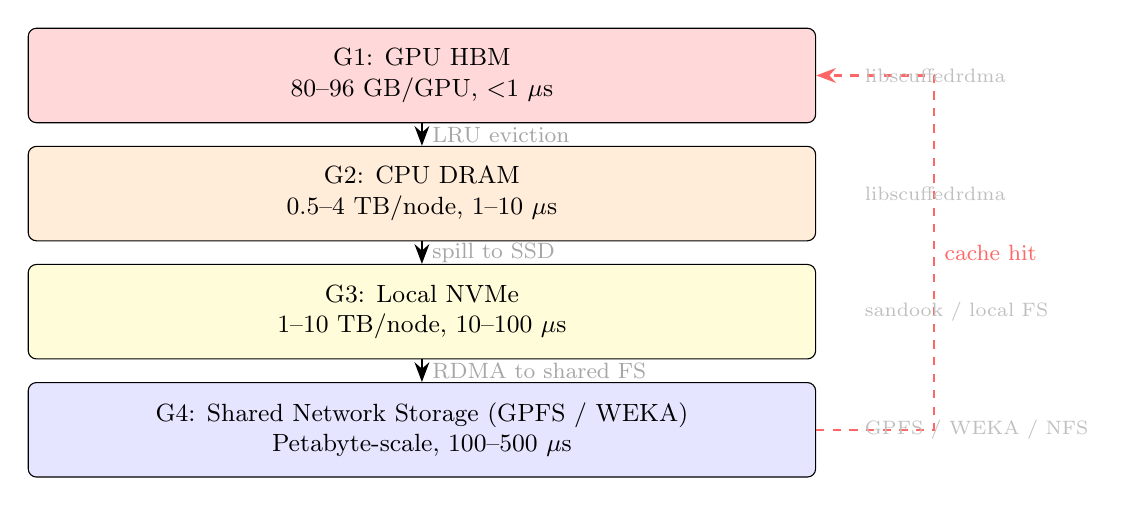
\begin{tikzpicture}[
    tier/.style={rectangle, draw, rounded corners=3pt, minimum width=10cm, minimum height=1.2cm, font=\small, align=center},
    arr/.style={-{Stealth[length=2.5mm]}, thick},
    lbl/.style={font=\footnotesize, text=gray!70}
]
\node[tier, fill=red!15] (g1) at (0, 4.5) {G1: GPU HBM\\80--96 GB/GPU, $<$1 $\mu$s};
\node[tier, fill=orange!15] (g2) at (0, 3.0) {G2: CPU DRAM\\0.5--4 TB/node, 1--10 $\mu$s};
\node[tier, fill=yellow!15] (g3) at (0, 1.5) {G3: Local NVMe\\1--10 TB/node, 10--100 $\mu$s};
\node[tier, fill=blue!10] (g4) at (0, 0.0) {G4: Shared Network Storage (GPFS / WEKA)\\Petabyte-scale, 100--500 $\mu$s};

\draw[arr] (g1) -- (g2) node[midway, right, lbl] {LRU eviction};
\draw[arr] (g2) -- (g3) node[midway, right, lbl] {spill to SSD};
\draw[arr] (g3) -- (g4) node[midway, right, lbl] {RDMA to shared FS};
\draw[arr, dashed, color=red!60] (g4.east) -- ++(1.5, 0) |- (g1.east) node[pos=0.25, right, font=\footnotesize, text=red!60] {cache hit};

\node[font=\scriptsize, text=gray!50, anchor=west] at (5.5, 4.5) {libscuffedrdma};
\node[font=\scriptsize, text=gray!50, anchor=west] at (5.5, 3.0) {libscuffedrdma};
\node[font=\scriptsize, text=gray!50, anchor=west] at (5.5, 1.5) {sandook / local FS};
\node[font=\scriptsize, text=gray!50, anchor=west] at (5.5, 0.0) {GPFS / WEKA / NFS};
\end{tikzpicture}
\caption{Four-tier KV memory hierarchy. libscuffedrdma currently handles G1--G2 transfers over RDMA. This update considers extending to G3 and G4.}
\label{fig:four_tier}
\end{figure}

The thesis so far operates at the G1--G1 boundary: KV moves between GPUs on different nodes. With a storage tier, the WFA classifier gains a third routing decision: not just hot QP vs cold QP, but also ``spill to storage'' vs ``transfer to peer.''

\section{GPFS Block Size Tradeoffs}

IBM Storage Scale (GPFS) is the reference enterprise parallel filesystem for this work. The block size configuration has direct consequences for KV cache workloads.

\subsection{Block Sizes, Subblocks, and Metadata}

GPFS allocates data in fixed-size blocks, typically 256 KB to 16 MB. Each block can be subdivided into \emph{subblocks} (1/32 of the full block by default) so that small files don't waste an entire block.

\begin{table}[ht]
\centering\small
\begin{tabular}{rrrrl}
\toprule
\textbf{Block size} & \textbf{Subblock} & \textbf{Metadata \%} & \textbf{ioctl/GB} & \textbf{Best for} \\
\midrule
256 KB & 8 KB & 3--5\% & $\sim$4000 & Small files, metadata-heavy \\
1 MB & 32 KB & 1--3\% & $\sim$1000 & General purpose (default) \\
4 MB & 128 KB & $<$1\% & $\sim$250 & Streaming large files \\
8 MB & 256 KB & $<$0.5\% & $\sim$125 & Bulk sequential writes \\
16 MB & 512 KB & $<$0.3\% & $\sim$63 & Maximum throughput \\
\bottomrule
\end{tabular}
\caption{GPFS block size tradeoffs. Larger blocks reduce metadata overhead and ioctl calls per GB transferred, but waste more space for small files. A 10-byte file in an 8 MB block wastes nearly 8 MB (subblocks partially mitigate this).}
\label{tab:block_sizes}
\end{table}

The engineering tradeoffs:

\begin{itemize}
\item \textbf{Larger blocks reduce metadata overhead.} Fewer blocks per GB means fewer metadata entries on disk and fewer ioctl calls to the kernel for memory mapping. Streaming reads and writes of large files run with lower CPU utilization because each syscall moves more data.
\item \textbf{Larger blocks waste more space for small files.} A 10-byte KV index entry in an 8 MB block wastes $\approx$8 MB minus 10 bytes. Subblocks help (a 256 KB subblock on an 8 MB block limits waste to 256 KB), but the overhead is still significant for metadata-heavy workloads.
\item \textbf{Don't change defaults without IBM support.} It is easy to make a configuration change that seems reasonable but opens up single points of failure or interacts badly with GPFS's internal metadata replication. The default 1 MB data block with 32 KB subblocks is safe for most workloads.
\end{itemize}

\subsection{KV Cache Block Alignment}

\noindent vLLM's PagedAttention~\cite{vllm_paged} uses 16-token KV blocks.
With 32 KV heads and head\_dim=128 at FP16, each block is about 256~KB.
scuffedQuant 3-bit compression ($\sim$5$\times$) shrinks that to about 50~KB.

\begin{table}[ht]
\centering\small
\begin{tabular}{lrrr}
\toprule
\textbf{KV format} & \textbf{Per-block} & \textbf{GPFS 1 MB} & \textbf{GPFS 4 MB} \\
\midrule
FP16 (uncompressed) & $\sim$256 KB & 4 blocks/alloc & 16 blocks/alloc \\
scuffedQuant 3-bit & $\sim$50 KB & 20 blocks/alloc & 80 blocks/alloc \\
\bottomrule
\end{tabular}
\caption{KV block alignment with GPFS block sizes. Compressed blocks are small enough that coalescing 20--80 blocks before a single GPFS write amortizes the allocation overhead.}
\label{tab:kv_alignment}
\end{table}

The practical implication: the cold QP should coalesce compressed KV blocks before flushing to the storage tier. Writing 50 KB blocks one at a time to GPFS wastes subblock granularity and multiplies ioctl overhead. Batching 20 compressed blocks into a single 1 MB write matches the default GPFS block size exactly.

\section{Sandook: Commodity NVMe Aggregation}

Sandook~\cite{sandook2026} (MIT, NSDI 2026) aggregates multiple NVMe SSDs into a unified Linux block device with read/write workload isolation. It targets the G3 tier: local SSD storage that is faster than network-attached GPFS but smaller in capacity.

\subsection{Architecture}

Sandook's key contribution is dynamic workload isolation. A control-plane scheduler profiles each SSD's load-latency curve offline. At runtime, client-side load balancers steer I/O to the least-loaded replicas, maintaining sub-millisecond p99 tail latency even under mixed read/write pressure.

This mirrors the WFA classifier's hot/cold split: sandook isolates read-heavy (cache hit) from write-heavy (cache spill) SSD traffic the same way libscuffedrdma isolates latency-critical metadata from bulk KV transfers. The difference is the layer: sandook operates at the block device, libscuffedrdma at the RDMA NIC.

\subsection{Relevance}

On a cluster without IBM Storage Scale licensing (like ours), sandook is a credible G3 tier. Each node could aggregate its local NVMe drives behind sandook, expose a block device, and the WFA classifier routes ``spill-to-local'' traffic to that device. Capacity is limited (1--10 TB per node), but latency is an order of magnitude lower than network storage.

\section{WEKA Augmented Memory Grid}

WEKA~\cite{weka2025amg} takes a different approach: a user-space real-time OS with kernel-bypass RDMA and consistent-hash metadata. Their Augmented Memory Grid (AMG) extends GPU memory capacity by 1000$\times$ using NVMe-backed KV storage with GPUDirect Storage (GDS) for zero-copy GPU-to-storage transfers.

Performance numbers from WEKA's benchmarks: 7.5M read IOPS, 1.0M write IOPS on an 8-node cluster. On 128K-token sequences they report 41$\times$ TTFT reduction, bringing prefill from 24 seconds to under 600 ms.

The tradeoff vs GPFS: WEKA is purpose-built for this workload and requires no block-size tuning (the filesystem handles it internally), but it is proprietary and requires specific hardware configurations. GPFS is more flexible and widely deployed but demands careful configuration.

\section{Dual QP Pool Extension to Storage}

\subsection{The Three-Way Classification}

The WFA classifier currently makes a binary decision: hot QP or cold QP. With a storage tier, this extends to a three-way decision:

\begin{enumerate}
\item \textbf{Hot QP} (network): small latency-critical metadata, scheduling decisions, attention-critical transfers. Same as Update 4.
\item \textbf{Cold QP} (network): bulk KV cache transfers between nodes. Same as Update 4.
\item \textbf{Storage spill}: KV blocks evicted from GPU memory, written to G3 (local NVMe via sandook) or G4 (GPFS via RDMA).
\end{enumerate}

The PMP controller's switching function generalizes: instead of allocating bandwidth between two QP pools, it allocates between network QPs and the storage path. When GPU memory pressure is low, all bandwidth goes to network transfers. When memory pressure rises, the controller diverts eviction traffic to the storage tier without blocking latency-critical transfers on the hot QP.

\subsection{Block Size Strategy}

The dual QP architecture naturally maps to GPFS block size recommendations:

\begin{table}[ht]
\centering\small
\begin{tabular}{lllll}
\toprule
\textbf{Traffic class} & \textbf{QP} & \textbf{GPFS block} & \textbf{Strategy} & \textbf{Why} \\
\midrule
KV index/metadata & Hot & 256 KB & Per-entry writes & Latency over throughput \\
Bulk KV spill & Cold & 1--4 MB & Coalesced batches & Amortize ioctl overhead \\
KV cache hit (read) & Hot & any & Direct read & Latency-critical retrieval \\
Checkpoint/snapshot & Cold & 8--16 MB & Streaming write & Maximum throughput \\
\bottomrule
\end{tabular}
\caption{Mapping traffic classes to GPFS block size strategy via the dual QP pool.}
\label{tab:storage_mapping}
\end{table}

This is not a recommendation to change GPFS block sizes. The default 1 MB block with 32 KB subblocks handles all four traffic classes. The point is that the WFA classifier's routing decision should account for the downstream block size: coalescing 20 compressed KV blocks into a 1 MB write before posting to the cold QP avoids subblock fragmentation on the storage side.

\section{GPUDirect Storage and BlueField-4}

NVIDIA's BlueField-4 DPU~\cite{bf4_cmx} offloads both the RDMA network path and the storage control plane from the host CPU. Combined with GPUDirect Storage (GDS), this enables a DMA path from GPU HBM directly to NVMe or network-attached storage without CPU involvement.

On our cluster (no BlueField, no ConnectX with GDS), this path is not available. KV spills go GPU $\to$ host DRAM $\to$ SoftRoCE $\to$ peer or storage. The CPU is in the loop for both the RDMA post and the storage write. This is the gap that makes the WFA's coalescing strategy important: without DPU offload, each ioctl has real CPU cost, and batching reduces that cost linearly.

For clusters with BlueField-4, the architecture simplifies: the DPU handles coalescing internally, and the WFA classifier only needs to decide ``network'' vs ``storage'' without worrying about block alignment. The dual QP split still matters for head-of-line blocking, but the storage path becomes a hardware concern rather than a software one.

\section{Measured NVMe Spill Throughput}

Before discussing GPFS and sandook deployment, we measured our local NVMe as a baseline. Compressed KV blocks (3-bit scuffedQuant, 256 tokens, 32 heads, head\_dim=128) land at 1.5~MB per block. We wrote and read them at different coalescing depths on Chimera's NVMe (\texttt{benchmarks/test\_arch/bench\_storage\_spill.py}).

\begin{table}[ht]
\centering\small
\begin{tabular}{rrrr}
\toprule
\textbf{Coalesce} & \textbf{Payload} & \textbf{Write} & \textbf{Read} \\
\midrule
1 block & 1.5 MB & 662 MB/s & 1,731 MB/s \\
10 blocks & 15.3 MB & 731 MB/s & 2,149 MB/s \\
20 blocks & 30.6 MB & 803 MB/s & 2,188 MB/s \\
50 blocks & 76.6 MB & 827 MB/s & 1,104 MB/s \\
\bottomrule
\end{tabular}
\caption{NVMe spill/retrieve throughput on Chimera. Coalescing 20 blocks hits the throughput plateau for writes and peak reads. 50 blocks drops read throughput due to page cache pressure.}
\label{tab:nvme_measured}
\end{table}

The 20-block sweet spot (30~MB per write) aligns with GPFS default 1~MB data blocks: 30 compressed blocks fit in 30 GPFS blocks, each below the subblock boundary. Our local NVMe at 803~MB/s write is about 10$\times$ slower than IBM Storage Scale's cited 8~GB/s. scuffedQuant's 6.4$\times$ compression narrows the effective gap: a compressed 803~MB/s path moves the same KV content as an uncompressed 5~GB/s path.

\section{Deployment Paths}

Two concrete paths for the storage tier are now accessible. Both have been confirmed to work on commodity hardware.

\subsection{IBM Storage Scale via Ansible}

IBM publishes an Ansible role collection for Storage Scale at \texttt{IBM/ibm-spectrum-scale-install-infra}~\cite{gpfs_ansible}. Relevant details:

\begin{itemize}
\item Supports Ubuntu 22 on x86\_64 (matches our Chimera/Cerberus setup).
\item Installs core GPFS packages, compiles the kernel extension (\texttt{mmbuildgpl}), creates the cluster, adds NSDs, and provisions a file system with a single Ansible run.
\item Deploys the management GUI, a Callhome service for support uploads, and the CES (Cluster Export Services) protocol nodes for SMB/NFS.
\item Includes prerequisite hardening: disables SELinux/firewall when asked, generates SSH keys, installs kernel-devel.
\end{itemize}

\paragraph{How we would use it.} A two-node GPFS cluster on Chimera/Cerberus using the Ansible role:

\begin{enumerate}
\item Each node exposes one NVMe partition as an NSD (Network Shared Disk).
\item Default block size 1~MB, metadata block 256~KB. Do not touch this without IBM support.
\item Create a single file system mounted at \texttt{/gpfs/scuffedrdma} on both nodes.
\item libscuffedrdma's cold QP spills coalesced 1~MB compressed KV batches to the file system.
\item The hot QP bypasses storage entirely: attention-critical traffic stays in-memory.
\end{enumerate}

This exercises the Update~4 dual-QP architecture against a real parallel file system rather than the idealized numbers from Hsu et al. The comparison that matters: our coalesced-write throughput versus GPFS's claim of sub-millisecond metadata and 8~GB/s data path. If we match within an order of magnitude on consumer hardware, the paper tells a stronger story about software-RDMA + compression as an alternative to enterprise storage.

\subsection{sandook for Commodity NVMe}

sandook~\cite{sandook2026} is the MIT NSDI 2026 artifact for aggregated NVMe with workload isolation. The GitHub repository provides a working prototype with a two-node QuickStart~\cite{sandook_quickstart}. The architecture is:

\begin{itemize}
\item \textbf{Controller} (central process): schedules reads/writes across SSDs using offline SSD performance profiles.
\item \textbf{Disk server} (per-SSD process): exposes the NVMe via SPDK or POSIX backend, reports IOPS/latency to the controller.
\item \textbf{Block device agent} (client side): uses \texttt{ublksrv} (userspace block device driver) to expose \texttt{/dev/ublkb0} to the host. Any file system can mount on top.
\item \textbf{Networking}: Caladan userspace TCP, runs on a dedicated NIC PCI address.
\item \textbf{Read/write isolation}: the controller dynamically partitions SSDs into read-heavy and write-heavy groups based on measured latency.
\end{itemize}

\paragraph{How we would use it.} A two-node sandook deployment on our cluster:

\begin{enumerate}
\item Cerberus runs the controller and a disk server over its local NVMe.
\item Chimera runs the block device agent, mounts \texttt{/dev/ublkb0} as ext4 at \texttt{/mnt/sandook}.
\item libscuffedrdma spills compressed KV blocks through \texttt{/mnt/sandook} rather than local NVMe. The sandook layer transparently aggregates both nodes' NVMe.
\item Run the same spill benchmark (Table~\ref{tab:nvme_measured}) with the sandook mount as the target. Expected effect: aggregated throughput from two NVMe drives, minus the Caladan+TCP overhead.
\end{enumerate}

\paragraph{Why sandook matches our design.} The sandook scheduler split (control plane at slow timescales for isolation decisions, data plane at fast timescales for per-request routing) mirrors the WFA + PMP split in libscuffedrdma. Both systems solve the same problem at different layers: WFA + PMP pick the right QP, sandook picks the right SSD. A combined deployment means the full stack from GPU HBM to persistent storage applies the same classify-then-route principle at every hop.

\paragraph{Dependencies.} sandook requires the \texttt{ublk} kernel driver (Linux 6.0+, Chimera/Cerberus run 6.8) and a Caladan-compatible NIC (most standard 10~GbE NICs work; the PCI address is configured explicitly). Neither is a blocker.

\subsection{GDS, WEKA, BlueField-4}

\begin{itemize}
\item \textbf{GPUDirect Storage (GDS)} requires \texttt{nvidia-peermem} which does not work with SoftRoCE (no NIC driver callbacks). Available only on Tower~2 with ConnectX-4.
\item \textbf{WEKA NeuralMesh} requires a licensed WEKA cluster. Their published numbers (41$\times$ TTFT reduction, 7.5M read IOPS) serve as the high-end comparison target.
\item \textbf{BlueField-4 DPU} handles coalescing and storage control-plane offload in hardware. Not on our testbed.
\end{itemize}

\section{Next Steps}

\begin{enumerate}
\item Deploy the IBM Ansible role against Chimera/Cerberus: create a two-node GPFS cluster, mount at \texttt{/gpfs/scuffedrdma}, run the spill benchmark, compare against the 803~MB/s local NVMe baseline.
\item Build sandook on both nodes following the QuickStart: controller on Cerberus, block agent on Chimera. Benchmark the aggregated NVMe throughput and sub-millisecond tail latency claim from the paper.
\item Implement KV spill/retrieve inside \texttt{middleware/rdma\_tensor\_cache/} with \texttt{aio\_write}/\texttt{aio\_read}, gated by the WFA classifier. Route a configurable fraction of cold-pool traffic to storage instead of the network.
\item Extend the PMP controller with a storage-pressure term based on GPU memory headroom.
\end{enumerate}

\begin{thebibliography}{99}

\bibitem{hsu2026kv}
A.~Hsu, K.~Ngo, Y.~Zhu, R.~Stoica, G.~Margalit, V.~Tarasov, and M.~Kieran, ``Rethinking LLM Inference Economics: KV Cache Reuse with llm-d, LMCache, and IBM Storage Scale,'' IBM Community, Feb.\ 2026.

\bibitem{hsu2026fourtier}
V.~Hsu, ``Accelerating NVIDIA Dynamo with IBM Storage Scale and BlueField-4 Inference Context Memory Storage Platform,'' IBM Community, Jan.\ 2026.

\bibitem{vllm_paged}
W.~Kwon et al., ``Efficient Memory Management for Large Language Model Serving with PagedAttention,'' \emph{Proc.\ SOSP}, 2023. arXiv:2309.06180.

\bibitem{sandook2026}
G.~I.~Chaudhry, A.~Bhardwaj, Z.~Ruan, and A.~Belay, ``Unleashing The Potential of Datacenter SSDs by Taming Performance Variability,'' \emph{Proc.\ NSDI}, 2026. \url{https://github.com/mit-sandook/sandook}

\bibitem{sandook_quickstart}
MIT sandook team, ``Sandook NSDI 2026 Artifact QuickStart,'' 2026. \url{https://github.com/mit-sandook/sandook/blob/main/nsdi-26-ae/QuickStart.md}

\bibitem{gpfs_ansible}
IBM, ``IBM Storage Scale (GPFS) Deployment using Ansible Roles,'' 2026. \url{https://github.com/IBM/ibm-spectrum-scale-install-infra}

\bibitem{weka2025amg}
WEKA, ``Augmented Memory Grid: Breaking the AI Memory Barrier,'' 2025. \url{https://www.weka.io}

\bibitem{bf4_cmx}
NVIDIA, ``Introducing NVIDIA BlueField-4 Powered Inference Context Memory Storage Platform,'' NVIDIA Developer Blog, 2026.

\bibitem{lmcache2025}
LMCache Team, ``LMCache: Enterprise KV Cache Management for LLM Serving,'' arXiv:2510.09665, 2025.

\bibitem{llmd_v05}
Red Hat, ``llm-d: Kubernetes-native Distributed LLM Inference,'' v0.5, 2025.

\bibitem{turboquant2026}
TurboQuant Team, ``TurboQuant: Online Vector Quantization for KV Cache Compression,'' 2026. arXiv:2504.19874.

\end{thebibliography}

\end{document}
